\documentclass[]{beamer}
% Class options include: notes, notesonly, handout, trans,
%                        hidesubsections, shadesubsections,
%                        inrow, blue, red, grey, brown

\usepackage[absolute,overlay]{textpos}
\setlength{\TPHorizModule}{1mm} \setlength{\TPVertModule}{1mm}
\newcommand{\MyLogo}{%
\begin{textblock}{14}(115.9,0.1)
  
\includegraphics[width=1.22cm]{kth_rgb}
 \end{textblock}
}


% Theme for beamer presentation.
\usepackage{beamerthemesplit} 
\usepackage{amssymb}
\usepackage{theorem}
\usepackage{graphicx} % Include figure files
\usepackage{epstopdf}
\usepackage{amsmath} % Include the ast symbol
\usepackage{comment}  % Include the comment function
\usepackage[english]{babel}
\usepackage[latin1]{inputenc}
\usepackage{tikz}
\usetikzlibrary{shapes,arrows}
% Other themes include: beamerthemebars, beamerthemelined, 
%                       beamerthemetree, beamerthemetreebars  
\title{Fitting of the effective mass}    % Enter your title between curly braces
\author{Rongzhen Chen}                 % Enter your name between curly braces
\institute{Royal Institute of Technology}      % Enter your institute name between curly braces
\date{January 14, 2013}                    % Enter the date or \today between curly braces


\begin{document}
\def\hath{\hat{H}}
\def\wf {\Psi(\{\bf{R}_\textit{I}, \bf{r}_\textit{i} \})}
\def\wfbo{\Psi_{\textit{bo}}({\textbf{r}_{\textit{i}}})}
\def\wfh{\Psi_{\textit{h}}({\textbf{r}_{\textit{i}}})}
\def\wfhit<#1>{\Psi_{\textit{h}}^{#1}({\textbf{r}_{\textit{i}}})}
\def\bwf<#1><#2>{\phi_{#1}(\textbf{r}_{#2})}
\def\wfbloch<#1><#2>{\Psi_{#1,#2}(\textbf{r})}
\def\ubloch<#1><#2>{u_{#1,#2}(\textbf{r})}
\def\ebloch<#1><#2>{E_{#1,#2}}
\def\bwfc<#1><#2><#3>{\phi_{#1}^{#3}(\textbf{r}_{#2})}
\def\sumi<#1> {\sum\limits_\textit{#1}}
\def\sumij<#1><#2> {\sum\limits_\textit{#1,#2}}
\def\suminj<#1><#2> {\sum\limits_{\textit{#1} \neq \textit{#2}}}
\def\coefkhe{-\frac{\hbar^2}{2 m_\textit{e}}}
\def\coefkhn{-\frac{\hbar^2}{2 M_\textit{I}}}
\def\nablai2<#1> {{\nabla}_{\textit{#1}}^{2}}
\def\moperater{-i\hbar \nabla}
\def\sumg<#1>{{\sum\limits_{\bf{#1}}}}    
\def\sumlm<#1><#2>{\sum\limits_{{#1}{#2}}}
\def\coeff<#1><#2><#3>{C_{#1,\bf{k_0}+\bf{#2}}^{#3}}      %C_{j,k_0+G}^{*}
\def\expkg<#1><#2>{e^{i(\bf{#1}+\bf{#2})\bf{r}}}          %exp{i(k+G)r}
\def\expg<#1>{e^{i\bf{#1}\bf{r}}}                         %exp{iGr}
%\def\bwf<#1>{\phi_{\bf{k_0}+\bf{#1}}^{\textbf{APW}}(\textbf{r})}          %phi_{k_0+G}  
\def\chig<#1>{{\chi_{\bf{kk_0}}(\bf{#1})}}                  %chi_{kk_0}{G}
%\def\hath{ | \hat{H} | }           
\def\kplusg<#1><#2>{(\bf{#1}+\bf{#2})}                    % k+G 
\def\radiaf<#1><#2>{f_{{\ell}^{\prime}{m}^{\prime}} (r_{\alpha},\bf{#1+#2})}    % f(r,k+G)
\def\radiafc<#1><#2><#3>{f_{{\ell}^{\prime}{m}^{\prime}}^{#3} (r_{\alpha},\bf{#1+#2})}    % f(r,k+G)
\def\bradiaf{u^{\alpha}_{q,\ell^{\prime}}(r_{\alpha},E_{\ell^{\prime}})}              %u(r_\alpha) did not contain the Energy
\def\sphfr<#1><#2><#3> {{Y_{#1}^{#3}(\hat{\bf{#2}}_{\alpha})}}                             %Y_{lm}(\hat{r})
\def\sphfq<#1><#2><#3> {{Y_{#1}^{#3}(\hat{\bf{#2}})}}                             %Y_{lm}(\hat{q})
\def\gaucoe{C_{{\ell{m}},{\ell^{\prime}m^{\prime}},{\ell^{\prime\prime}m^{\prime\prime}}}}  %Gaunt coefficient
\def\potvgir{V_{\bf{G^{\prime\prime}}}}                                %V{G}
\def\potvmt{V^{\alpha}_{{\ell}^{\prime\prime}{m}^{\prime\prime}} (r_{\alpha})}  %V{lm,r}   
\def\fracatom<#1> {e^{i\bf{#1}\bf{R^\alpha}}}   % exp(iqR)
\def\bessf<#1>{j_{\ell}({#1}r_{\alpha})}     %j_l(kr)
\def\dr{\mathrm{d}\bf{r}}
\def\chikp<#1><#2>{{\chi_{#1,#2}(\textbf{r})}}  
\MyLogo



% Creates title page of slide show using above information
\begin{frame}
  \titlepage
\MyLogo
\end{frame}
\note{Talk for 30 minutes} % Add notes to yourself that will be displayed when
                           % typeset with the notes or notesonly class options

\section[Outline]{}

\begin{frame}

 \tableofcontents

\MyLogo
\end{frame}


\section{Backgroundaaa}
\begin{frame}
\MyLogo
In solid state physcis, the effective mass is defined as follows:

\begin{equation}
 \frac{1}{m^*_{\alpha\beta}} = \frac{1}{\hbar^2} \frac{d^2 E(\textbf{k} )}{dk_\alpha dk_\beta}
\end{equation}

where $m^*$ is effective mass, and $E(k)$ is the band dispersion relation between energy $E$ and $k$. 
And the effective mass reflects the band curvature, the flatter of band, the larger effective mass.
\end{frame}

\begin{frame}
\MyLogo
In this report, I will fit the effective mass around the $\Gamma$ point for the semiconductor material $CuInSe_2$ by taking advantage of least-squares fitting in Python.

Energy $E$ is as follows:
\begin{equation}
 E = \frac{\hbar^2}{2m^*_{xy}} (k^2_x+k^2_y)+ \frac{\hbar^2}{2m^*_z} (k^2_z)
\end{equation}

which means that we want to know the value $m^*_{xy}$ and $m^*_{z}$ by given the value of $E$ and  $k_x, k_y$ and $k_z$.
\end{frame}


\section{Program Flow} 
\begin{frame}
\MyLogo
%%%%%%%%%%%%%%%%%%%%figure
\tikzstyle{decision} = [diamond, draw, fill=white!20,
    text width=10em, text badly centered, node distance=2.5cm, inner sep=0pt]
\tikzstyle{block} = [rectangle, draw, fill=white!20,
    text width=12em, text centered, rounded corners, minimum height=3em]
\tikzstyle{line} = [draw, very thick, color=black!50, -latex']

\begin{figure}[!htb]
\centering

\begin{tikzpicture}[scale=0.4 , node distance = 2.5cm,transform shape]
    % Place nodes
    \node [block] (init) {Reading band dispersion};
    \node [block, below of=init] (orig) {Plot original band dispersion};
    \node [block, below of=orig] (fitting) {Fitting band dispersion};
    \node [block, below of=fitting] (plotf) {Plot fitting result};
    \node [block, left of=plotf, node distance=6cm] (update) {Re-fitting};
    \node [decision, below of=plotf, node distance=3.8cm] (converge) {Original==Fitting};
    \node [block, below of=converge, node distance=3.8cm] (done) {Finished};
    % Draw edges
    \path [line] (init) -- (orig);
    \path [line] (orig) -- (fitting);
    \path [line] (fitting) -- (plotf);
    \path [line] (plotf) -- (converge);
    \path [line] (converge) -| node [near start, color=black] {No} (update);
    \path [line] (update) |- (fitting);
    \path [line] (converge) -- node [, color=black] {Yes}(done);

\end{tikzpicture}
\caption{Flow chart of fitting energy band dispersion}
\end{figure}


\end{frame}



\section{Result}
\begin{frame}
\MyLogo
Here are the results from fitting, I compare my fitting results (value inside the parentheses in red color) with the paper [C. Persson, Appl. Phys. Lett. 93, 072106 (2008)], where I find out there are quite similar, so the code is 
reliable to be used.

\begin{table}[ht]
\caption{Effective mass for $CuInSe_2$}
% title of Table
\centering
% used for centering table
\begin{tabular}{c c c c c}
% centered columns (4 columns)
\hline\hline 
%inserts double horizontal lines
  & $c$1 & $v$1 & $v$2 & $v$3\\ [0.5ex]
% inserts table
%heading
\hline \\
% inserts single horizontal line
         $m_{xy}$ & 0.08 ({\color{red}0.08}) & 0.14 ({\color{red}0.13}) & 0.25 ({\color{red}0.25})& 0.27 ({\color{red}0.26})\\
% inserting body of the table
$m_z$ & 0.09 ({\color{red}0.09}) & 0.66 ({\color{red}0.65}) & 0.12 ({\color{red}0.12})& 0.28 ({\color{red}0.28})\\[0.1ex]
% [1ex] adds vertical space
\hline
%inserts single line
\end{tabular}
\label{table:nonlin}
% is used to refer this table in the text
\end{table}

\end{frame}

\begin{frame}
\MyLogo
And following figures are the fitting result from $v$1 as one example, also with testing results.

\begin{figure}[H]
     \begin{center}
            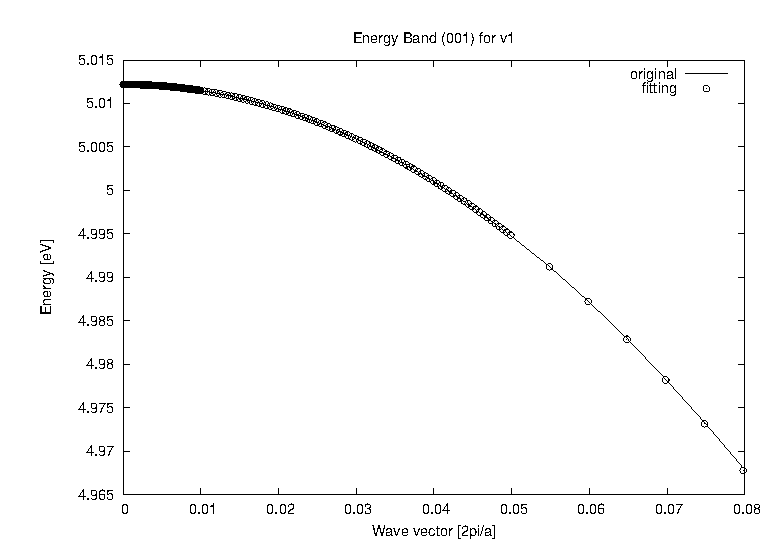
\includegraphics[width=0.5\textwidth]{mz126.eps}
            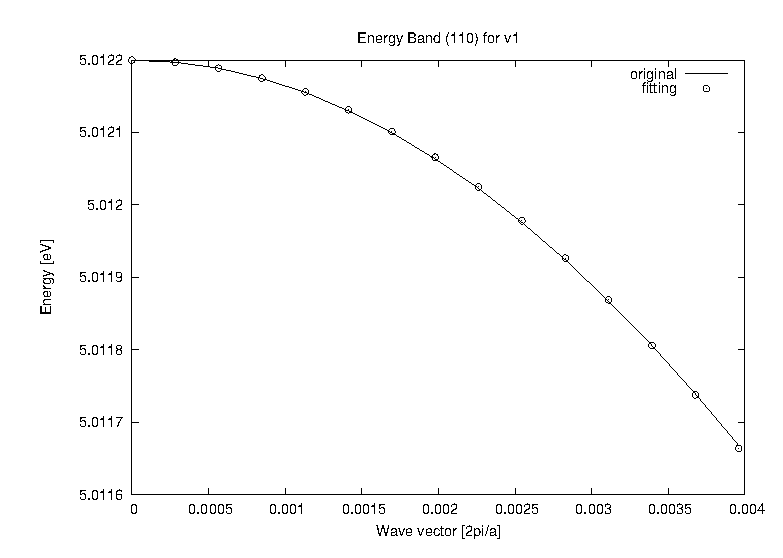
\includegraphics[width=0.5\textwidth]{mxy126.eps}
     \end{center}
    \caption{Fitting results for band $v$1}
\end{figure}
\end{frame}

\begin{frame}
\MyLogo
\begin{figure}[H]
     \begin{center}
            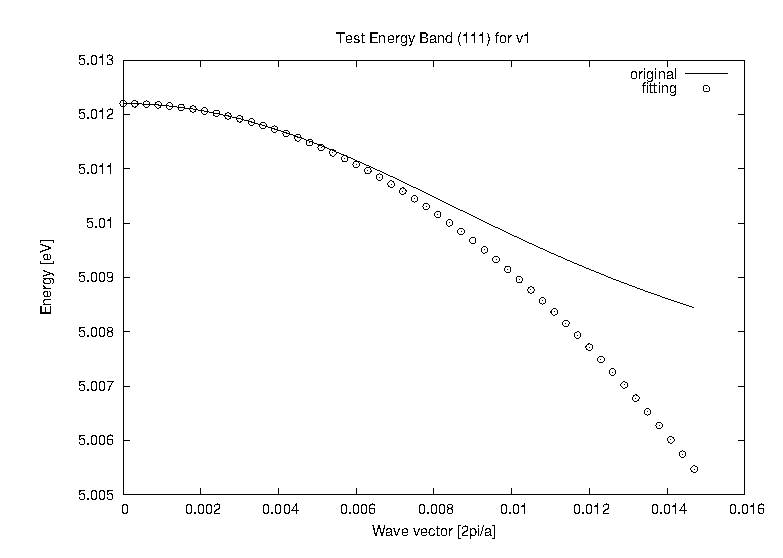
\includegraphics[width=0.5\textwidth]{test111bandindex126.eps}
            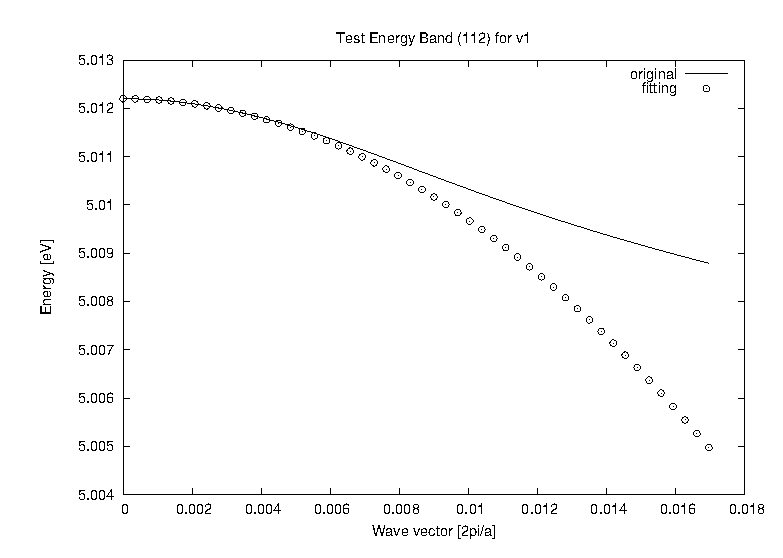
\includegraphics[width=0.5\textwidth]{test112bandindex126.eps}
     \end{center}
    \caption{Testing results for band $v$1}
\end{figure}
\end{frame}


\section{Future}
\begin{frame}
\MyLogo
 There are several places I can improve this code, for example, I can creat a graphical user interface to convenient user, or make this code more flexible, or find the maximum valence band index automatically. 
\end{frame}


\begin{frame}
\MyLogo
\begin{center}
 \Huge Thank you for your time!
\end{center}
\end{frame}



\end{document}
